\section{仪器响应简介}
地震仪观测到的地面运动记录可以表示为
\[  u(t) = s(t) * g(t) * i(t) \]
其中$s(t)$代表震源项,$g(t)$代表路径效应,$i(t)$代表仪器响应,星号代表卷积。
翻译成中文就是``地面运动记录是震源项、路径项以及仪器响应三者的卷积''。

四个量中:
\begin{itemize}
\item $u(t)$是地震仪的数字记录,已知;
\item $i(t)$在仪器设计的时候会给出各种参数,已知;
\item $s(t)$为震源项,包括震源机制、震源时间函数等,未知;
\item $g(t)$为路径项,即地球内部结构,未知。
\end{itemize}
其中的两个未知项,是地震学研究的两个主要内容:震源和结构。
因而理解仪器响应$i(t)$的基本原理并准确地去除仪器响应是研究的关键一步。

真实世界里,有很多因素会引起地面的运动,比如地震波、长周期潮汐波以及
人类活动等等,因而真实的地面运动是极其复杂的。图 \ref{fig:ground-motion}
给出了COLA台站记录到的持续时间为 \SI{22000}{\s} 左右的地面运动情况,
即$s(t)*g(t)$所对应的波形:

从图 \ref{fig:ground-motion} 可以看到,整个地面运动中最明显的地方是
弯弯曲曲类似正弦的波形,其周期大概在 \SI{6000}{\s},也就是两个小时,
这很可能是潮汐波引起的长周期地面运动。波形的最大振幅大概是 \num{2e7}。
在 \SI{1000}{\s} 左右有一个明显的振动信号,这是一个震级为Mw \num{8.3}
级的大地震的信号,其振幅大概在 \num{2e6} 的量级,比长周期波小了一个量级。

这就是真实的地面运动。即便是如此大的地震,其引起的地面运动相对来说也是
很小的。这样的记录因为有太多其它类型的地面运动的干扰,因而对于地震学来
说是没有太大用处的,所以就需要设计合适的仪器尽量去除其它类型地面运动的
干扰,也就是地震仪。

\begin{figure}[H]
\centering
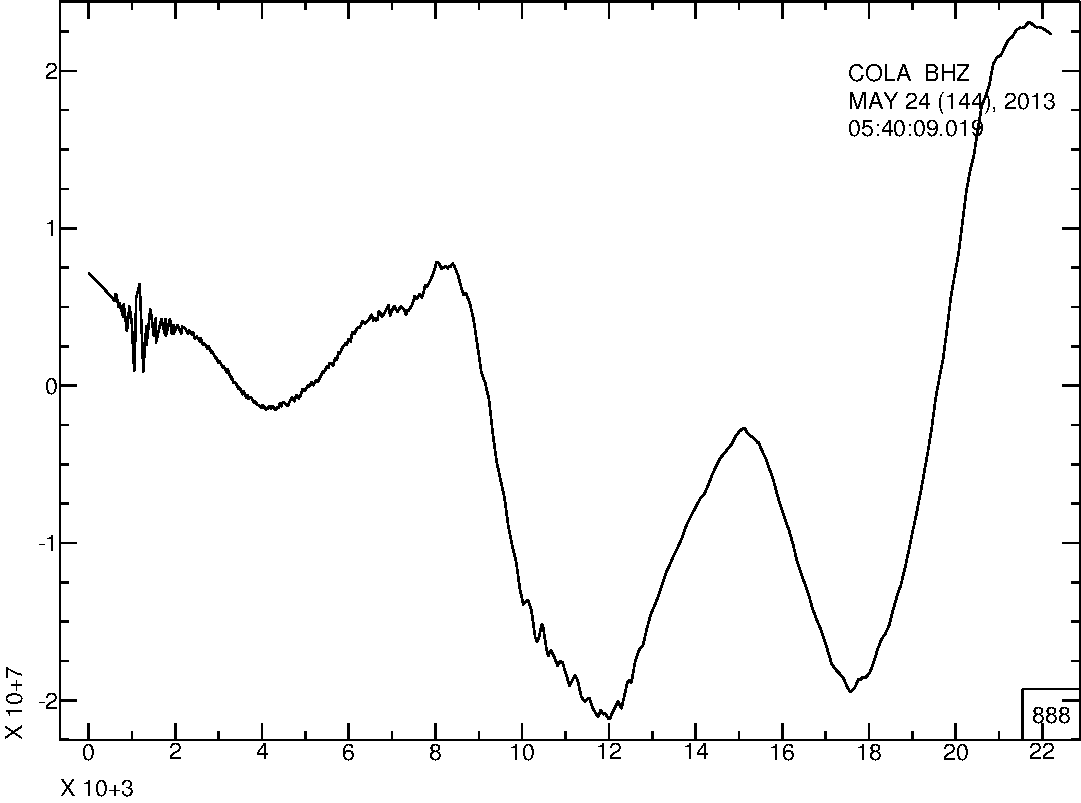
\includegraphics[width=0.98\textwidth]{ground-motion}
\caption{COLA台站处的原始地面运动}
\label{fig:ground-motion}
\end{figure}

从信号处理的角度来看,常见的地震仪是一个带通滤波器,对地震学不关心的
超高频和超低频的信号进行压制,只保留感兴趣的周期段。下图给出了该台站的
仪器响应,即$i(t)$:

\begin{figure}[H]
\centering
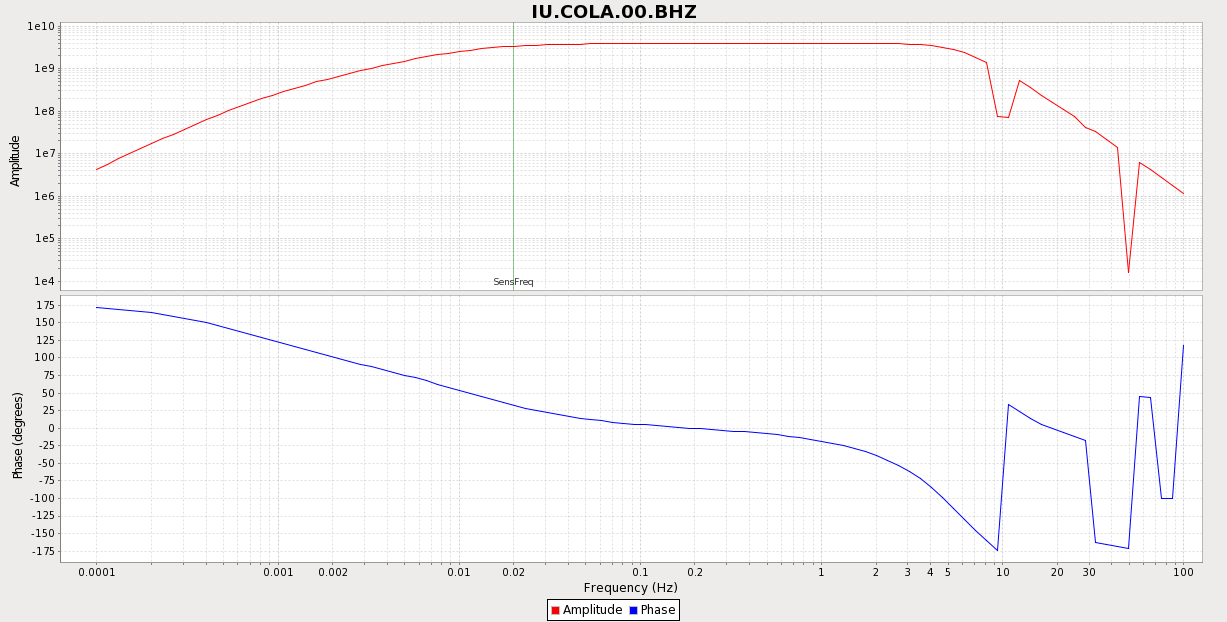
\includegraphics[width=0.98\textwidth]{transfer-function}
\caption{仪器响应频谱图}
\label{fig:transfer-function}
\end{figure}

\begin{figure}[H]
\centering
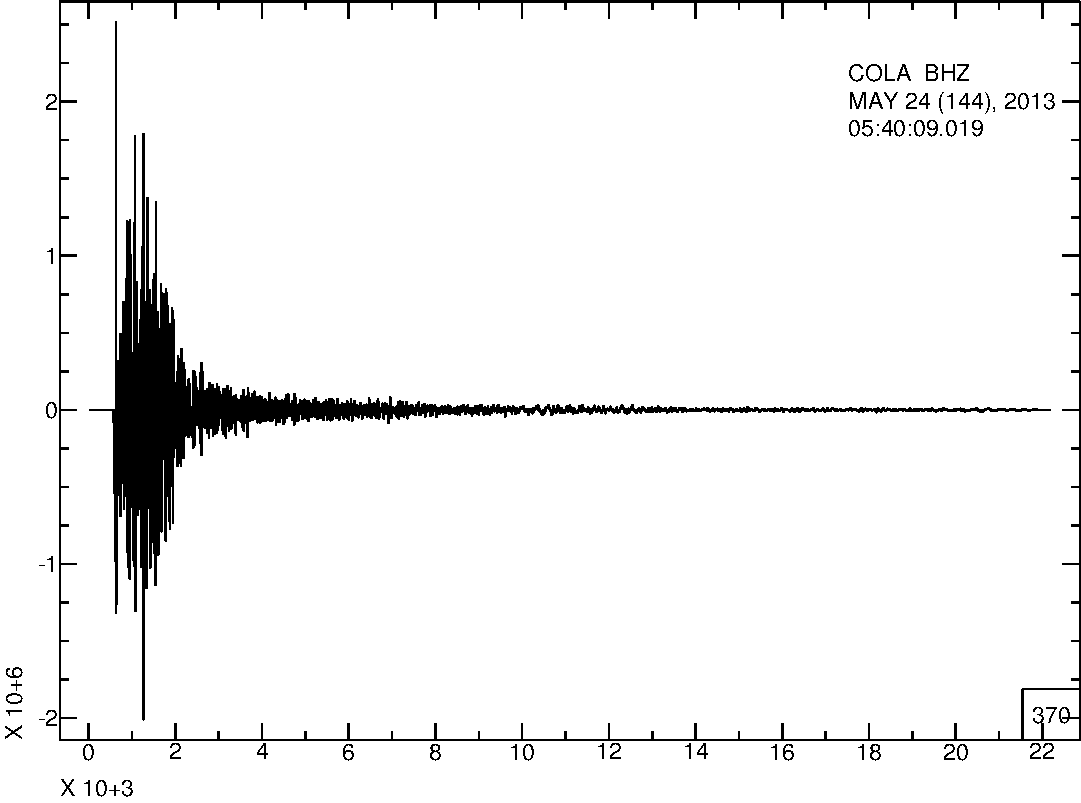
\includegraphics[width=0.9\textwidth]{raw-data}
\caption{COLA台站的地震记录}
\end{figure}

从图 \ref{fig:transfer-function} 中振幅谱可以看出,频率在 \SI{0.02}{\Hz}
到 \SI{8}{\Hz} 内的信号具有相同的振幅增益(被增强),而小于 \SI{0.02}{\Hz}
或大于 \SI{8}{\Hz} 的信号则被压制。图 \ref{fig:ground-motion} 中的周期为
\SI{1000}{\s} 量级的信号被压制到了原来的千分之一。

原始的地面运动$s(t)*g(t)$在经过仪器$i(t)$之后,即得到地震仪的数字记录,如下图。
超低频和超高频的信号被压制,留下地震学感兴趣的频段,也就是前面说的$u(t)$:

与图 \ref{fig:ground-motion} 相比,长周期的类正弦信号没了。在 \SI{0}{\s}
到 \SI{300}{\s} 内,``地面''很安静,\SI{300}{\s} 左右,强烈的地震信号
开始出现,最大振幅约为 \num{2.4e6},持续了很长一段时间后,又恢复了``平静''。
这里可以很明显地看到``平静$\rightarrow$震动$\rightarrow$平静''的过程。这才是地震数据处理理想的波形。

为什么要去仪器响应呢?哪些时候需要去仪器响应呢?下面列举出若干需要
去仪器响应的场景:
\begin{itemize}
\item 需要获取某个台站绝对振幅值;
\item 仪器响应不同的台站之间的波形对比;
\item 待补充...
\end{itemize}
